\documentclass[a4paper,12pt]{article}
\usepackage{graphicx}
\usepackage[left=2.5cm, right=2.5cm, top=3cm, bottom=3cm]{geometry}
\usepackage{amsmath, amsthm, amssymb}
\usepackage[spanish]{babel}
\usepackage{url}
\begin{document}
\title{Informe sobre el proyecto Moogle}
\author{Abraham Romero Imbert}

\date{Julio, 2023}
\maketitle
\begin{abstract}
En este informe se estará explicando de manera más detallada el funcionamiento del Proyecto Moogle!. Se interiorizará la ejecución del mismo así como en las clases y métodos que intervienen en el proceso para dar una respuesta al usuario, una vez hecha una consulta.
\end{abstract}
\section{Introducción}\label{sec:intro}
Es el primer proyecto de Programación orientado a Primer Año de Ciencias de la Computación. Básicamente es una aplicación cuyo propósito es buscar inteligentemente un texto en un conjunto de documentos. Como cualquier buscador busca información en una base de datos a partir de palabras clave o frases que el usuario introduce en la barra de búsqueda. Utiliza algoritmos para encontrar archivos que contienen las palabras clave y las presenta al usuario en una lista de resultados teniendo en cuenta la relevancia de los mismos respecto a la búsqueda realizada. Adicionalmente este buscador tiene la capacidad de sugerir al usuario otras posibles búsquedas, en especial al no encontrar resultados en la base de datos semejantes a la petición inicial del usuario.

\section{Funcionamiento}

\subsection{Ruta de ejecución}\label{subsec:ejec-rut}

Dentro del \texttt{namespace} \textbf{MoogleEngine} y utilizando la biblioteca \textbf{System.IO}; dentro de la clase estática \textbf{Moogle} busco la ruta dinámica(desde donde se encuentra el proyecto) y se ejecuta el programa y analizando cada archivo de la carpeta \textbf{Content} (ubicada en la carpeta raíz) almaceno los nombres de los archivos en un \texttt{string [ ]}.

\subsection{Clase: \textbf{Diccionario-Referencial}}\label{subsec:dic-ref}

Luego creo un objeto estático de mi clase \textbf{Diccionario-Referencial}. Esta clase crea un \texttt{diccionario} que contiene información sobre la ocurrencia de las palabras en documentos y su posición en una matriz de índices. El constructor toma una \texttt{string [ ]} de archivos de texto como entrada y realiza varias operaciones en cada archivo para crear el diccionario. Primero, tokeniza el contenido del archivo en palabras separadas por delimitadores. Luego, cuenta la cantidad de palabras en cada documento y las agrega al diccionario \textbf{Cant-pal-DOC}. También asigna un índice de fila a cada documento en el diccionario \textbf{Indexador-Fila}. A continuación, para cada palabra en el archivo, agrega una entrada al diccionario \textbf{Indexador-Columnas} si no existe ya, y agrega la palabra al diccionario \textbf{Ocurrencia-de-i-en-documentos} si tampoco existe. Si la palabra ya existe en el diccionario, incrementa su valor de ocurrencia en 1(una vez por cada documento donde aparezca). Finalmente, establece la cantidad de archivos procesados en la variable \textbf{Cant-arch}. También hay un método \textbf{Tokenizar-txt} que toma una ruta de archivo o una cadena de texto como entrada y devuelve un \texttt{string [ ]} de palabras tokenizadas.

\subsection{Clase: \textbf{Matriz-TF-IDF}}\label{subsec:matriz-TF-IDF}

Luego creo un objeto estático  de la \texttt{clase} \textbf{Matriz-TF-IDF}.  Esta tiene dos métodos: el constructor y \textbf{Respuesta-query}. También
tiene una propiedad \textbf{matriz} formada por un \textbf{Vector} \texttt{[ ]}

Es importante explicar antes en que consiste la clase  \textbf{Vector}:

\subsubsection{Clase: Vector}\label{subsubsec:Vector}

\textbf{Vector} representa un vector en \textbf{Matriz-TF-IDF} como un \texttt{double [ ]}. Tiene varios métodos:

\begin{enumerate}

\item El constructo: toma como entrada un objeto \textbf{Diccionario-Referencial} y un \texttt{string} que representa el archivo correspondiente al vector. Crea un nuevo vector y lo inicializa con ceros. Luego, itera sobre las palabras en el archivo y actualiza el vector con los valores \textit{TF-IDF} correspondientes para cada palabra.
\item El segundo constructor: toma como entrada un \texttt{double [ ]} que representa un \textit{query} y crea un nuevo vector con esos valores.
\item El método \textbf{Calculo-TF-IDF} calcula el valor \textit{TF-IDF} para una palabra en un documento específico, utilizando la fórmula siguiente:

\begin{equation}\label{eq:TF*IDF}
TF\cdot IDF
\end{equation}

Donde 

\begin{equation}\label{eq:TF}
TF_{i}=\frac{\log_{2}(Freq(i,j)+1)}{\log_{2}(L_{j}+0.001)}
\end{equation}

Freq(i,j)+1 = Frecuencia del término i en el documento j.

$L_{j}$ = Número total de términos en el documento j. En este caso se le sumo a este valor 0.001 para evitar indefiniciones en la función 

\begin{equation}\label{eq:IDF}
IDF_{i} = log_{2}(1+\frac{N_{d}}{f_{i}+1})
\end{equation}
$N_{d}$= Número total de documentos considerados\\
$f_{i}$ = Número de documentos que contienen el término i. En este caso se le sumo a este valor 1 para evitar indefiniciones en la función 

\item El \textit{método} \textbf{Multiplicar-por-Vector} calcula el \textit{producto punto} entre dos vectores.
\item \textbf{Norma} calcula la \textit{norma} del vector.
\item \textbf{Cosigno} calcula el \textit{coseno} entre dos vectores.

Este viene determinado por la fórmula siguiente y representa la semejanza que existen entre dos documentos (incluido la \textit{query}) este valor viene oscila entre 0 y 1 donde 0 representa que ambos documentos son \textit{ortogonales} o sea no tienen palabras en común y 1 que son documentos con las mismas ocurrencias de palabras una vez normalizados, claramente mientras más cercano sea el valor de \textit{coseno} a 1 más similares serán los documentos.   

\begin{equation}
\cos(\theta) = \frac{A\cdot B}{\parallel A\parallel \* \parallel B\parallel}= \frac{\sum\limits_{i=1}^n A_i\* B_i}{\sqrt{\sum\limits_{i=1}^n A_i^2}\* \sqrt{\sum\limits_{i=1}^n B_i^2}}
\end{equation}

\end{enumerate}

\subsection{Continuación Clase: \textbf{Matriz-TF-IDF}}\label{subsec:cont-matriz-TF-IDF}

Luego volviendo a la clase \textbf{Matriz-TF-IDF}:
El \textit{constructor} toma como entrada un objeto \textbf{Diccionario-Referencial} y la \textit{ruta} donde se encuentran los documentos. Crea un \textbf{Vector} \texttt{[ ]}, donde cada vector representa una fila en la matriz. Luego, itera 
sobre el \texttt{diccionario} de índices de fila en el objeto \textbf{Diccionario-Referencial} y crea un nuevo objeto \textbf{Vector} para cada fila en la matriz. Este toma como entrada el \textit{objeto} \textbf{Diccionario-Referencial} y el índice de fila correspondiente. Finalmente, agrega el vector a la matriz.

El \textit{método} \textbf{Respuesta-query} toma como entrada un objeto \textbf{Query-class} de la clase con el mismo nombre, un objeto \textbf{Matriz-TF-IDF} y un objeto \textbf{Diccionario-Referencial}. Itera sobre el diccionario de índices de fila en el objeto \textbf{Diccionario-Referencial} y calcula el coseno entre el vector de consulta (almacenado en el objeto \textbf{Query-class}) y cada fila en la matriz (almacenada en el objeto \textbf{Matriz-TF-IDF}). Agrega los resultados al diccionario \textbf{Solution}, que contiene los nombres de los documentos y sus puntajes de similitud con la consulta. Si \textbf{Solution} tiene más de 5 elementos, elimina el documento con el puntaje más bajo (utilizando el método \textbf{Menor}). Luego, elimina cualquier entrada en \textbf{Solution} que tenga un puntaje de similitud igual a cero. Finalmente, ordena \textbf{Solution} por puntaje de similitud y lo devuelve como un nuevo diccionario llamado \textbf{orderedSolution}.

El método estático \textbf{Menor} toma como entrada un diccionario de \texttt{string} y \texttt{double} y devuelve la clave del par con el valor más bajo.

Luego está el \textit{método estático} \textbf{Query} el cual dado un \textit{query} devuelve un objeto \textbf{SearchResult}.Para esto primeramente se crea un textbf{SearchResult} \texttt{[ ]} items así como un objeto que representa al \textit{query} de mi clase \textbf{Query-class}. 

\textbf{Query-class} se utiliza para representar el \textit{query} y trabajar con él. El \textit{constructor } de la clase recibe como parámetros el \textbf{Diccionario-Referencial} y el \texttt{string} \textbf{query}.
El método \textbf{Snippet} se encarga de generar un fragmento de texto que contenga las 
palabras más relevantes de la consulta en el contexto del documento. Para ello, primero se \textit{tokeniza} el documento y se identifican las palabras que coinciden con 
las de la consulta. Luego se ordenan estas palabras según su relevancia (calculada mediante el método \textbf{TF-IDF}) y se seleccionan las dos más relevantes. A continuación, se busca la posición más cercana de estas dos palabras en el documento (método \textbf{posicion-mas-cercana}) y se determina la vecindad de cada una (es decir, las palabras que la rodean, método \textbf{Vecindad}). Si la distancia entre ambas vecindades es mayor a 7 palabras, se retorna un fragmento que incluye ambas vecindades separadas por puntos suspensivos. Si la distancia es menor o igual a 7, se retorna un fragmento que incluye ambas vecindades sin puntos suspensivos. En resumen, el método \textbf{Snippet} genera un fragmento de texto que contiene las palabras más relevantes de la consulta en el contexto del documento, lo que puede ayudar al usuario a entender mejor cómo se relaciona su consulta con el contenido.

Además están los métodos:
\textbf{Busqueda-valida}: Ve si el \textit{query} es válido, sino devuelve algo así:

\begin{figure}[h]
    \center
    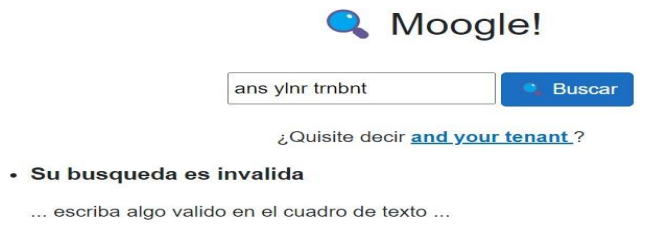
\includegraphics[width=8cm]{suggestion.png}
    \caption{Sugerencia en Moogle!}
    \label{fig:suggestion}
\end{figure}

Para la sugerencia usé los siguientes métodos: 
\textbf{LevensteinsDistance}: La \textit{distancia de Levenshtein} o distancia entre palabras es el número mínimo de operaciones requeridas para transformar un cadena de caracteres en otra. Se entiende por operación, bien una inserción, eliminación o la sustitución de un carácter. Este método calcula dicha distancia.
\textbf{MostSimilarWord}: Devuelve la palabra más parecida (menor \textit{distancia de Levensteins}) a la que se ingresa.
\textbf{Suggestion}: Devuelve un \textit{query}, sustituyendo las palabras inválidas por sus más parecidas. 
Luego a través del método \textbf{Busqueda-valida} se verifica si el \textit{query} es válido y si lo es se crea un diccionario con los documentos más relevantes y su respectivo \textit{score} (este diccionario le da la dimensión a \textit{items}) Luego se inicializa cada elemento de 
\textbf{SearchItems} \texttt{[ ]} items incluyendo su \textit{snippet}
Al final se hace una \textit{sugerencia} (método \textbf{Suggestion}) del \textit{query} y se devuelve un 
objeto \textbf{SearchResult} que se imprime en el \large{Moogle}.

\section{Conclusión}\label{sec:conclu}

En este informe se ha explicado detalladamente el código implementado por mí para la ejecución del Moogle!. Se han detallado las clases y los métodos propios de cada una, así como la manera en que se ejecutan estos, o sea, cómo funcionan. En vista de la posibilidad de un posterior mejoramiento de la capacidad de procesamiento de este proyecto o la implementación de otras funcionalidades se expresa que los métodos anteriores pueden estar sujetos a cambios. En mi experiencia particular este como mi primer proyecto en la Facultad de Matemática y Computación en la Universidad de la Habana considero que fue un gran paso en el tránsito del desconocimiento en la programación a este nuevo y amplio mundo donde \large{TODO} es posible. Quisiera agradecer a mis profesores y profesores de clases prácticas que cumplieron en su labor para aclarar mis dudas respecto al proyecto y me dieron herramientas para poder trabajar de manera más eficiente en su desarrollo, a ellos y demás personas que intervinieron muchas gracias.

\end{document}
 

